%第3章



本章では,V字開発モデルによる要求定義,基本設計,詳細設計について述べる.3.1節ではユースケース図を用いて,商品識別システムの要求定義を述べる.3.2節ではクラス図を用いて,商品識別システムの基本設計について述べる.3.3節ではシーケンス図を用いて商品識別システムの詳細設計を述べる.


\section{要求定義}


商品識別システムがどのように機能すべきかという振る舞いと,その外部環境を表した図\ref{usecase1}を載せる.

\begin{figure}[htbp]
\centering
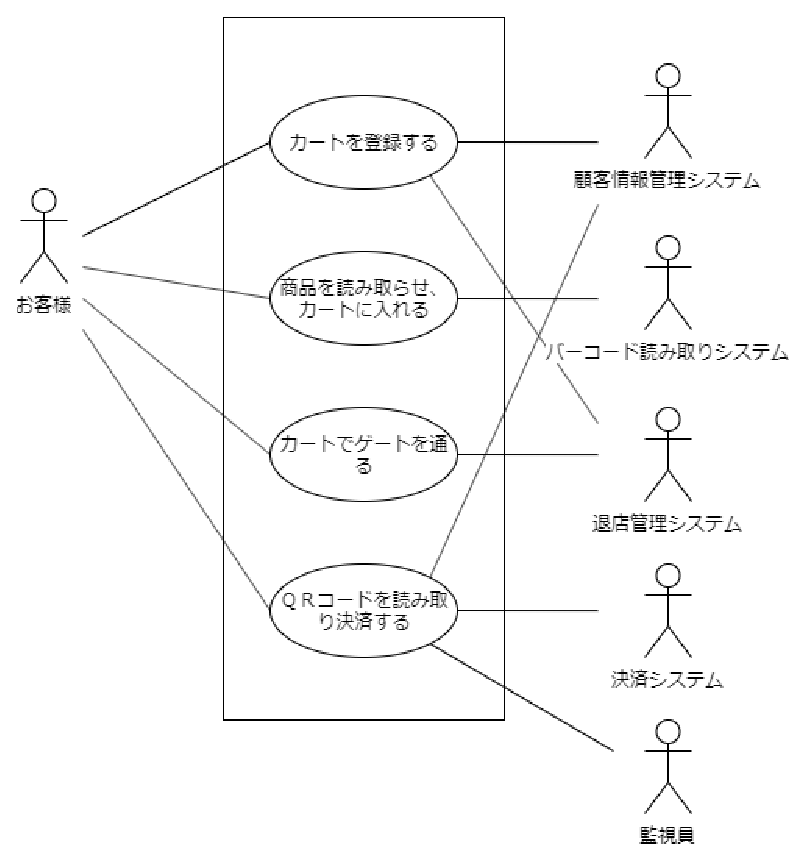
\includegraphics[width=15cm]{picture/usecase1.eps}
\caption{システムのユースケース図(1)}
\label{usecase1}
\end{figure}


\section{基本設計}

\section{詳細設計}